\chapter{Cleaning Robot: Learning Multiple User Preferences}

In order for a robot to clean an entire house or office, it would have to be able to fully understand its environment and make decisions based on the state of each room. For example, the robots can learn least occupancy time of the environment to make decisions on cleaning time which causes minimum interference for humans. In this chapter the robot will learn multiple user's preference in using different rooms of a office and determine the low occupancy time for cleaning.

\cite{Fink2013} did a exhaustive survey about usage, adoption process and long-term effects of domestic cleaning robot in people's homes. One of the biggest barrier for better adoption of robots in household was compatibility with habits and routines. 

\todo[inline]{Complete this }

\section{Hierarchical Beta Bernoulli Model}

Hierarchical beta bernoulli model as explained in \ref{chap: object} is used to model the occupancy of each room. The probabilistic graphical model is shown in Figure \ref{bbm2}

\noindent
\begin{figure}[htp]

\begin{minipage}{0.3\textwidth}
\centering

\tikz {
 % Define nodes
  \node[latent]                                 (theta) {$\theta$};
  \node[latent, above=of theta, xshift=-1.2cm]  (alpha) {$\alpha$};
  \node[latent, above=of theta, xshift=1.2cm]   (beta) {$\beta$};
  \node[obs, below=of theta]                    (y)     {$x$}; 
  % Connect the nodes
  \edge {alpha,beta} {theta} ; %
  \edge {theta} {y};
  % plates
  \plate {location} {(y)} {location};
  \plate {time} {(theta)(y)(location)} {time};
}

\end{minipage}%
\begin{minipage}{0.7\textwidth}

\begin{equation*}
	\alpha \sim Beta(2,2) ; \beta \sim Beta(2, 2);
\end{equation*}
\begin{equation*}
	\theta \sim Beta(\alpha, \beta);
\end{equation*}
\begin{equation*}
	x = Bernoulli(\theta)
\end{equation*}
\end{minipage}
\caption[Hierarchical Beta Bernoulli graphical model]{Graphical model representation of Hierarchical Beta Bernoulli model. The boxes are ``plates" representing replicates. The outer plates represents hours of a day, while the inner plate represents if the room has users in that hour.}
\label{bbm2}
\end{figure}



The model can be explained as:

	\boldmath{$\alpha$} and \boldmath{$\beta$} is  prior beta distribution, 
	
	$\theta_i$ is the latent occupancy distribution for period $i$  ,
	
	$x_{ij}$ is the observation in period $i$.

\section{Brayford Dataset}

Brayford dataset is extracted from the Witham Wharf RGB-D dataset, both collected as part of the Spatio-Temporal Representations and Activities for Cognitive Control in Long-Term Scenarios (STRANDS) project. 
Witham Wharf RGB-D dataset is used for testing RGB-D localization in changing environments. The dataset consist of RGB-D images collected over eight locations in an open-plan office. The Brayford dataset was extracted from the above dataset by manually annotating the presence of human in the room at the moment.

The dataset is divided in 2 parts the training set and testing set. The training set consist of 7 days of observations, where the robot visits predefined eight locations of the office at a regular interval of 10 minutes each. The testing set consist of another week of observation. 

The training dataset was used to learn the parameters of the model while the testing dataset was used to predict and validate the learned models. 



\begin{figure}[htp]
\centering
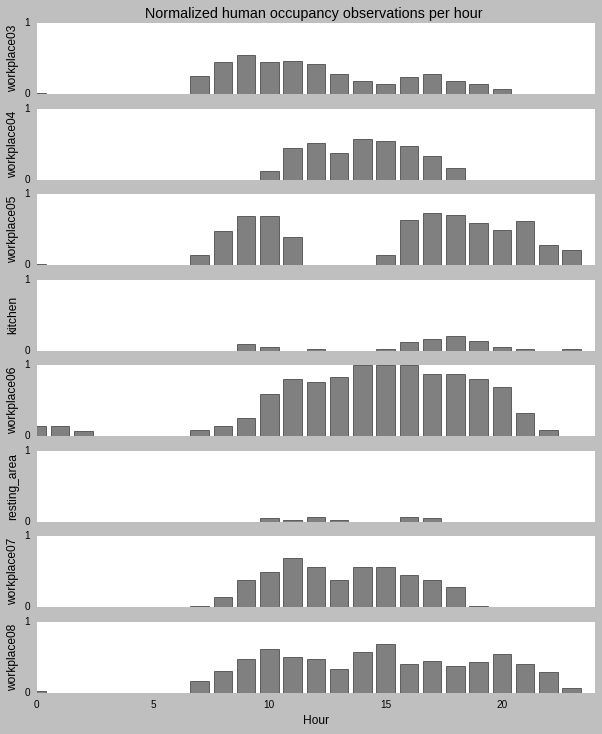
\includegraphics[width=\textwidth]{images/brayford_dataset_visualization.png}
\caption[Normalized human occupancy per hour]{Normalized human occupancy per hour: Number of }
\label{}
\end{figure}

\section{Evaluation and Discussions}

The dataset was evaluated using bootstrap methods. The models are learned on the training dataset. 



